\documentclass[12pt]{article}\usepackage[]{graphicx}\usepackage[]{color}
%% maxwidth is the original width if it is less than linewidth
%% otherwise use linewidth (to make sure the graphics do not exceed the margin)
\makeatletter
\def\maxwidth{ %
  \ifdim\Gin@nat@width>\linewidth
    \linewidth
  \else
    \Gin@nat@width
  \fi
}
\makeatother

\definecolor{fgcolor}{rgb}{0.345, 0.345, 0.345}
\newcommand{\hlnum}[1]{\textcolor[rgb]{0.686,0.059,0.569}{#1}}%
\newcommand{\hlstr}[1]{\textcolor[rgb]{0.192,0.494,0.8}{#1}}%
\newcommand{\hlcom}[1]{\textcolor[rgb]{0.678,0.584,0.686}{\textit{#1}}}%
\newcommand{\hlopt}[1]{\textcolor[rgb]{0,0,0}{#1}}%
\newcommand{\hlstd}[1]{\textcolor[rgb]{0.345,0.345,0.345}{#1}}%
\newcommand{\hlkwa}[1]{\textcolor[rgb]{0.161,0.373,0.58}{\textbf{#1}}}%
\newcommand{\hlkwb}[1]{\textcolor[rgb]{0.69,0.353,0.396}{#1}}%
\newcommand{\hlkwc}[1]{\textcolor[rgb]{0.333,0.667,0.333}{#1}}%
\newcommand{\hlkwd}[1]{\textcolor[rgb]{0.737,0.353,0.396}{\textbf{#1}}}%

\usepackage{framed}
\makeatletter
\newenvironment{kframe}{%
 \def\at@end@of@kframe{}%
 \ifinner\ifhmode%
  \def\at@end@of@kframe{\end{minipage}}%
  \begin{minipage}{\columnwidth}%
 \fi\fi%
 \def\FrameCommand##1{\hskip\@totalleftmargin \hskip-\fboxsep
 \colorbox{shadecolor}{##1}\hskip-\fboxsep
     % There is no \\@totalrightmargin, so:
     \hskip-\linewidth \hskip-\@totalleftmargin \hskip\columnwidth}%
 \MakeFramed {\advance\hsize-\width
   \@totalleftmargin\z@ \linewidth\hsize
   \@setminipage}}%
 {\par\unskip\endMakeFramed%
 \at@end@of@kframe}
\makeatother

\definecolor{shadecolor}{rgb}{.97, .97, .97}
\definecolor{messagecolor}{rgb}{0, 0, 0}
\definecolor{warningcolor}{rgb}{1, 0, 1}
\definecolor{errorcolor}{rgb}{1, 0, 0}
\newenvironment{knitrout}{}{} % an empty environment to be redefined in TeX

\usepackage{alltt}
\usepackage[lmargin =1in,rmargin=1in,tmargin =1in, bmargin =1in]{geometry}                
\geometry{letterpaper}               
\usepackage{graphicx}
\usepackage{subcaption}
\usepackage{multirow}
\usepackage{amssymb} \usepackage{fancyhdr}
\usepackage[affil-it]{authblk}
\usepackage{booktabs}
\usepackage{tabularx}
\usepackage{natbib}
\setlength{\headheight}{15.2pt}
\pagestyle{fancy}
\fancyhead{} % delete current setting for header
\fancyhead[C]{\noindent Notes from December \hfill Carles Boix }
%\linespread{1.6}
%% for inline R code: if the inline code is not correctly parsed, you will see a message
\newcommand{\rinline}[1]{SOMETHING WRONG WITH knitr}







\begin {document}
\section{Notes}
\subsection{12/28}
\textbf{MIG1}:
ATF only experiences the effect of increase in stress response which we have seen maps perfectly to other ATFs. Therefore, there is something there that we must look at; possibly construction; possibly preparation. Furthermore, when we look at MIG1, which appears to have a strong signal, we get a strong signal for the RAP1, MSN2, and MIG1 motifs in the ATF but only for MIG1 in the ZEV construct. 

When I take the top 200 from each and join them, the signal is in MIG1 and MSN2 (32 genes only, many HXT). I will need to look at the motifs specifically for these proteins, but they are very promising. However, only six of these genes are actually MIG1 targets as reported by SGD. Room for discovery? I need to look into this more specifically\footnote{13 are MSN2 targets (SGD), and of the 6 MIG targets, 3 are MSN2 targets; these two TFs seem to work together; maybe I can say something about the relationship?}.

We need to look at this in another way: \emph{where are the genes with motifs that match MIG1?} Are they distributed more upward in ATF than ZEV? and of course are they up/down regulated relative to baseline?\\


\textbf{MSN2}:
In the case of the top targets from ATF and ZEV for MSN2, we see \textbf{NO} difference between all genes and MSN2 at any time point for ATF, except for between 0 and 90u, where there may be a slight decrease (crowded out by other genes?)\footnote{Maybe another type of metric; not top 200 is in order?}. The merged list, that is, the genes in the top 200 in ATF and ZEV, has an increased occurrence of the MSN2 motif. This is certainly an interesting observation.\\


For ZEV, there is a difference, if slight. I need to try to look at where the genes with motifs corresponding to MSN2 are placed on this.\\

\textbf{RAP1}:
Nothing to say today. This may be the key to eliciting data from the 0-15 fold changes, but even that is unlikely. Let's just leave this alone until we have to discuss problems with the data, as it is the data set that will yield the clearest data on the ATF.\\

\textbf{With respect to code}:
I compiled a single table with all of the motif occurrences (above .25 occupancy)\footnote{Refer to Marcus for this} for each of the genes. It is quite sparse, which is good if I later want to do some groupwise analysis.

\subsection{12/29}
Beware of the expert curated motifs! The one for MSN2 is $\sim 5$ bases long, while the one for Rap1 is 13 bases. I show this in the following motifs logos (Figures~\ref{fig:logo1} and~\ref{fig:logo2}):

\begin{knitrout}
\definecolor{shadecolor}{rgb}{0.969, 0.969, 0.969}\color{fgcolor}\begin{figure}[]


{\centering 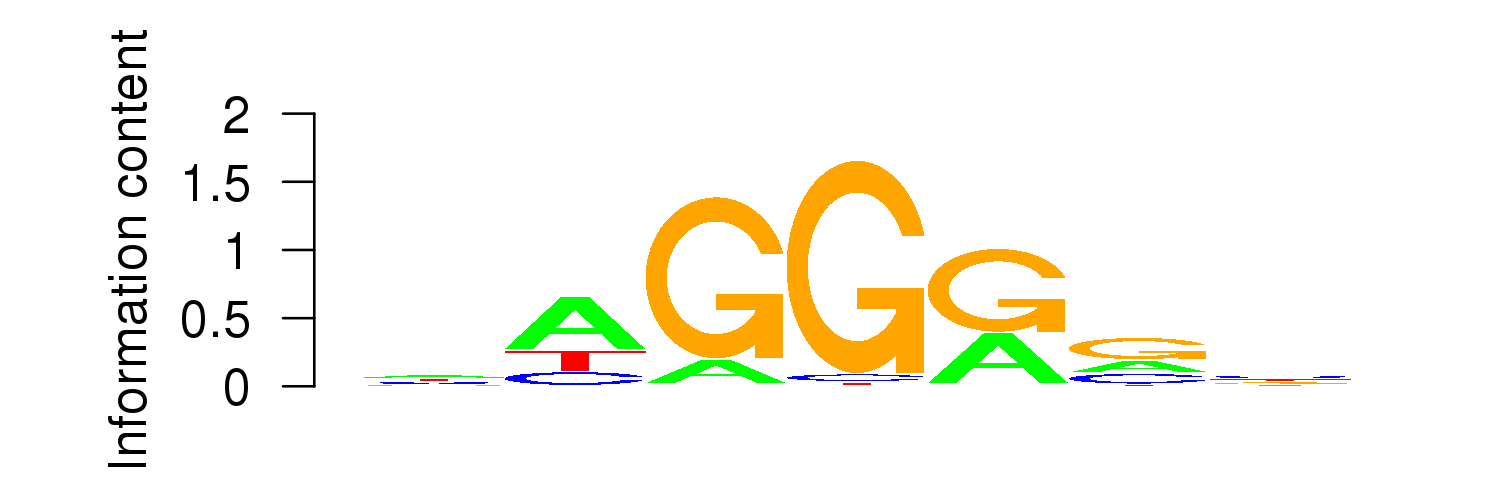
\includegraphics[width=.9\textwidth]{figure/latex-logo1} 

}

\caption[MSN2]{MSN2\label{fig:logo1}}
\end{figure}


\end{knitrout}


\begin{knitrout}
\definecolor{shadecolor}{rgb}{0.969, 0.969, 0.969}\color{fgcolor}\begin{figure}[]


{\centering 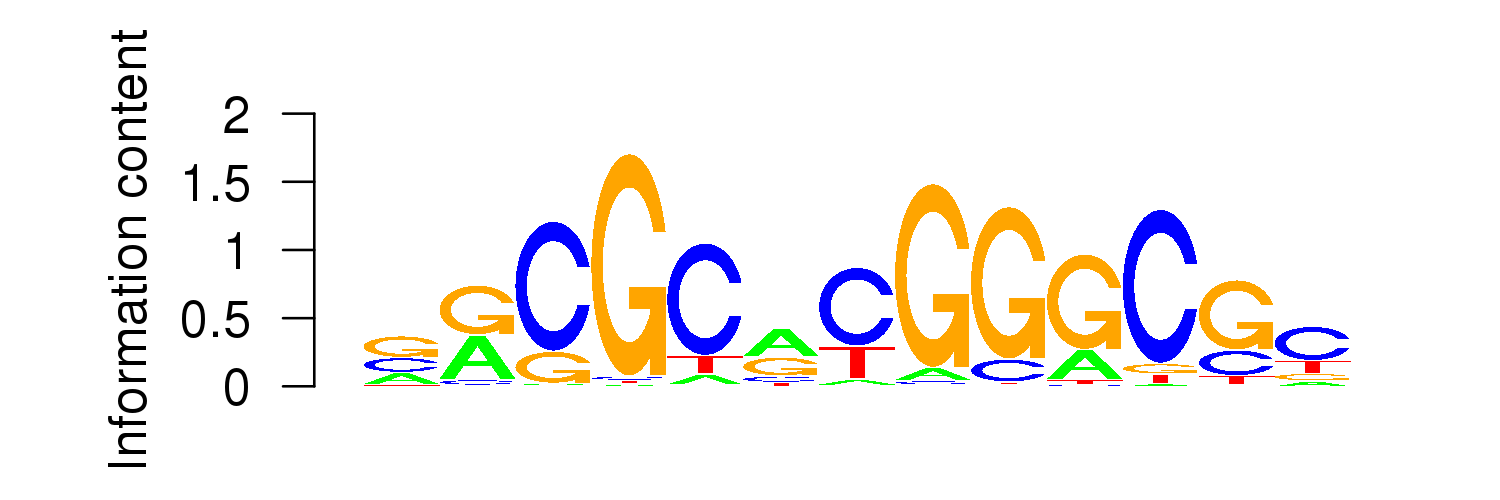
\includegraphics[width=.9\textwidth]{figure/latex-logo2} 

}

\caption[RAP1]{RAP1\label{fig:logo2}}
\end{figure}


\end{knitrout}


\end{document}
